\question(20分){已知控制系统结构图如下所示,求 $\frac{E_1(s)}{R(s)},\frac{E_2(s)}{R(s)},E_1(s),E_2(s)$

\begin{tikzpicture}[scale=1, thick]
\tikzstyle{block} = [draw,rectangle,thick,minimum height=1em,minimum width=1em]
\tikzstyle{sum} = [draw,circle,inner sep=0mm,minimum size=2mm]
\tikzstyle{branch} = [inner sep=0pt,minimum size=0pt]
\tikzstyle{connector} = [->,thick]
\matrix[ampersand replacement=\&, row sep=1em, column sep=1em]{
\&  \&  \& \node(n1){$N_1(s)$};\&\&\node(n2){$N_2(s)$}; \\

\&  \&  \node[block](g1){$\dfrac{1}{s}$}; \& \node[sum](p1) {}; \& \node[block] (g2){$\dfrac{1}{s}$}; \& \node[sum](p2) {};  \\

\node[] (r) {$R(s)$}; \& 
\node[branch] (b1) {} ; \&
\&
\node[sum](p3) {}; \&
\node[] (e1) {$E_1(s)$} ; \&
\&
\node[sum](p4) {};\&
\node[branch] (b2) {} ;  \&
\node[] (e2) {$E_2(s)$} ; 
\\

\& \node[sum](p5) {}; \&  \node[block](g3){$\dfrac{1}{s}$}; \&  \& \node[block](g4){$\dfrac{1}{s}$}; \&  \\
\& \& \& \node[block](h){$1+s$}; \\
};
\draw [connector] (n1) -- (p1);
\draw [connector] (n2) -- (p2);
\draw [connector] (b1) |- (g1);
\draw [connector] (r) -| (p5);
\draw [connector] (p5) -- (g3);
\draw [connector] (g1) -- (p1);
\draw [connector] (p1) -- (g2);\draw [connector] (p1) -- (p3);
\draw [connector] (g3) -- (g4);\draw [connector] (g3) -| node[very near end,left]{$-$}(p3);
\draw [connector] (p3) -- (e1);
\draw [connector] (g2) -- (p2);
\draw [connector] (p2) -| (p4);
\draw [connector] (g4) -| node[very near end,left]{$-$}(p4);
\draw [connector] (p4) -- (e2);
\draw [connector] (b2) |- (h);
\draw [connector] (h) -|  node[very near end,left] {$-$} (p5);
\end{tikzpicture} 

\onlyanswer
{
答:
\begin{align*}
E_1(s) &= N_1(s)+\frac{R(s)}{s}-\frac{R(s)-(1+s)E_2(s)}{s}\\
E_2(s) &= N_2(s)+\frac{R(s)}{s^2}+\frac{N_1(s)}{s}-\frac{R(s)-(1+s)E_2(s)}{s^2}
\end{align*}
化简得:
\begin{align*}
E_1(s) &= N_1(s)+\frac{(1+s)E_2(s)}{s} \\
E_2(s) &= N_2(s)+\frac{N_1(s)}{s}+\frac{(1+s)E_2(s)}{s^2}
\end{align*}
可得:
\begin{align*}
\frac{E_1(s)}{R(s)} &=0 \\
\frac{E_2(s)}{R(s)} &=0 \\
E_2(s)(1-\frac{1+s}{s^2}) &= N_2(s)+\frac{N_1(s)}{s} \\
E_2(s) &= \frac{N_2(s)+\frac{N_1(s)}{s}}{1-\frac{1+s}{s^2}} \\
 &= \frac{N_2(s)s^2+N_1(s)s}{s^2-s-1} \\
E_1(s) &= N_1(s)+\frac{(1+s)E_2(s)}{s} \\
 &= \frac{N_1(s)s^2+(1+s)sN_2(s)}{s^2-s-1}
\end{align*}
}

}

%\onlytest{\vskip 3em}

%\onlytest{\newpage}

\question(20分)已知控制系统模型如下:
\begin{align*}
\dot{y}(t) & =v(t) \\
\dot{v}(t) & =u(t) \\
u(t) &=e(t)-k_1 v(t)+k_2 \dot{r}(t)\\
e(t) &=r(t)- y(t)
\end{align*}
求传递函数  $G(s)=\frac{Y(s)}{R(s)}$,其中$Y(s)={\cal L}[y(t)],R(s)={\cal L}[r(t)]$ ;零初始条件下,$k_2=0,r(t)=1,(t>0)$时,为使系统超调量$\sigma\%=0$ ,且调节时间尽可能小, $k_1$应取何值? 零初始条件下,$r(t)=t,(t>0)$ 时,$k_1,k_2$取何值可使 $\lim_{t\rightarrow\infty}e(t)=0$  ?

\onlyanswer
{

答:

系统结构图:

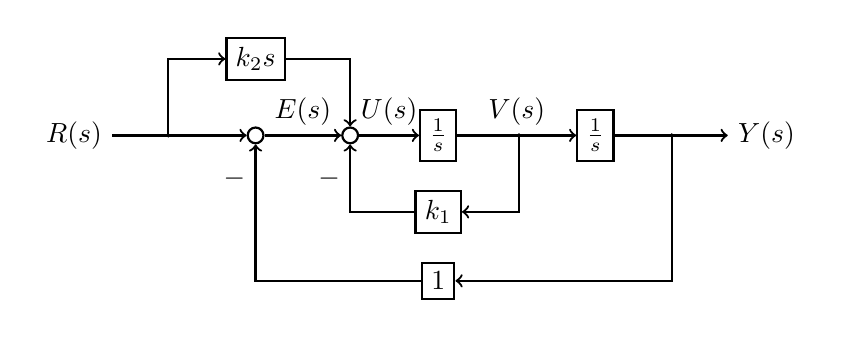
\begin{tikzpicture}[scale=1, thick] 
\tikzstyle{block} = [draw,rectangle,thick,minimum height=1em,minimum width=1em]
\tikzstyle{sum} = [draw,circle,inner sep=0mm,minimum size=2mm]
\tikzstyle{branch} = [draw,circle,fill,inner sep=0pt,minimum size=0.5pt]
\tikzstyle{connector} = [->,thick]
\matrix[ampersand replacement=\&, row sep=1em, column sep=2em]{
\& \&  \node[block](gr){$k_2 s$};\\
\node(r){$R(s)$};\&\node[branch](br){};\&\node[sum](pe){};\& \node[sum](pu){};\&\node[block](guv){$\frac{1}{ s}$};\&\node[branch](bv){};\&\node[block](gvy){$\frac{1}{s}$};\&\node[branch](by){};\& \node(c){$Y(s)$}; \\

\& \&\&\& \node[block](k1){$k_1$};\\
\& \&\&\& \node[block](h){$1$};\\
};

\draw [connector] (r) -- (pe);
\draw [connector] (br) |-(gr);
\draw [connector] (pe) -- node[midway,above] {$E(s)$}(pu);
\draw [connector] (gr) -|(pu);
\draw [connector] (pu) -- node[midway,above] {$U(s)$}(guv);
\draw [connector] (guv) -- node[midway,above] {$V(s)$}(gvy);
\draw [connector] (gvy) --(c);
\draw [connector]( bv) |-(k1);
\draw [connector] (k1) -| node[near end,left] {$-$} (pu);
\draw [connector] (by) |-(h);
\draw [connector] (h) -| node[very near end,left] {$-$} (pe);
\end{tikzpicture} 

由梅森公式,得:
\begin{align*}
G(s) &=\frac{\frac{k_2}{s}+\frac{1}{s^2}}{1+\frac{k_1}{s}+\frac{1}{s^2}} \\
 &=\frac{1+k_2 s}{s^2+s k_1+1}
\end{align*}

当系统为临界阻尼与过阻尼时,满足 $\sigma\%=0$, 临界阻尼调节时间小于过阻尼,因此

$$k_1=2\zeta\omega_n=2\cdot 1\cdot 1=2$$

零初始条件下, $r(t)=t,R(s)=\frac{1}{s^2}$ 时,
\begin{align*}
E(s) &=R(s)-G(s)R(s) \\
 &=\frac{s^2+k_1 s -k_2 s}{s^2+k_1 s+1}\cdot \frac{1}{s^2}
\end{align*}
当 $k_1>0$ 时系统稳定,且有:
\begin{align*}
\lim_{t\rightarrow\infty}e(t) &= \lim_{s\rightarrow 0}sE(s) \\
 &=k_1-k_2
\end{align*}
因此,当$k_1>0,k_1=k_2$时可使 $\lim_{t\rightarrow\infty}e(t)=0$
}
\question(20分)控制系统结构图如下:

\begin{tikzpicture}[scale=1, thick] 
\tikzstyle{block} = [draw,rectangle,thick,minimum height=1em,minimum width=1em]
\tikzstyle{sum} = [draw,circle,inner sep=0mm,minimum size=2mm]
\tikzstyle{branch} = [draw,circle,fill,inner sep=0pt,minimum size=0.5pt]
\tikzstyle{connector} = [->,thick]
\matrix[ampersand replacement=\&, row sep=1em, column sep=2em]{
\node(r){$R(s)$};\&\node[sum](pe){};\& \node[block](g){$\dfrac{s+1}{(s^2+as+b)(s+2)}$};\&\node[branch](bc) {} ; \& \node(c){$C(s)$}; \\

\& \& \node[block](gc){$1$};\\
};

\draw [connector] (r) -- (pe);
\draw [connector] (pe) -- node[midway,above] {$E(s)$} (g);
\draw [connector] (g) -- (c);
\draw [connector] (bc) |- (gc);
\draw [connector] (gc) -| node[near end,left] {$-$} (pe);
\end{tikzpicture} 

已知$a\geq 0,b\geq 0$,当$R(s)=\frac{1}{s}$时系统的稳态误差是多少?是否可通过改变$a,b$的值使得$R(s)=\frac{1}{s^2+1}$时稳态误差等于零?

\onlyanswer
{
答:
系统特征方程:
$$ s^3+(a+2)s^2 +(b+2a+1)s+2b+1=0 $$
劳斯表:
$$
\begin{matrix}
s^3 &  1       &  b+2a+1   \\
s^2 & (a+2) & 2b+1 \\
s^1 & b+2a+1-\frac{(2b+1)}{a+2} \\
s^0 & 2b+1 \\
\end{matrix}
$$
当$a\geq 0,b\geq 0$时,
\begin{align*}
 b+2a+1-\frac{(2b+1)}{a+2}&=\frac{ (a+2)*(b+2a+1)-(2b+1)}{a+2} \\
 &=\frac{ab+2a^2+5a+1}{a+2} \\
 &> 0
\end{align*}
系统稳定,可得:
\begin{align*}
E(s) &=\frac{(s^2+as+b)(s+2)}{(s^2+as+b)(s+2)+s+1}\cdot R(s) \\
\lim_{s\rightarrow 0} sE(s)&=\frac{2b}{2b+1}
\end{align*}
当 $R(s)=\frac{1}{s^2+1}$时
\begin{align*}
E(s) &=\frac{(s^2+as+b)(s+2)}{(s^2+as+b)(s+2)+s+1}\cdot \frac{1}{s^2+1}\\
&=\frac{s+2}{(s^2+as+b)(s+2)+s+1}\cdot\frac{s^2+as+b}{s^2+1} \\
\end{align*}
当$a=0,b=1$时,
\begin{align*}
E(s) &=\frac{s+2}{(s^2+as+b)(s+2)+s+1} \\
\lim_{t\rightarrow\infty}e(t) &=\lim_{s\rightarrow 0} sE(s)\\
&=0
\end{align*}
}

\question  (20分) 单位负反馈系统开环传递函数
$$G(s)=\frac{k}{s(s+1)^3}$$
绘制 $k\in(-\infty,0)\cup(0,\infty)$的系统根轨迹,并分析系统稳定时 $k$ 的取值范围。

\onlyanswer
{
答:
系统开环极点:$(-1+0j),0$, 渐近线中心:$\frac{-1-1-1}{4}=\frac{-3}{4}+0j$,
分离点:
\begin{align*}
\frac{\mathrm{d}}{\mathrm{d}s}(s(s+1)^3+k) &=0 \\
(s+1)^3+3s(s+1)^2 &=0\\
(s+1)^2(s+1+3s) &=0
\end{align*}
因此分离点为$-1,(\frac{-1}{4}+0j)$ 。
利用劳斯判据求根轨迹与虚轴交点:
$$
\begin{matrix}
s^4 & 1           & 3   & k \\
s^3 & 3           & 1       \\
s^2 & \frac{8}{3} & k
\end{matrix}
$$
$k=\frac{8}{9}$ 时可得辅助方程: $\frac{8}{3}s^2+k=0$ ,解得: $s=\pm\frac{\sqrt{3}}{3}j$ 。

$k\in(0,\infty)$ 时, 实轴上的根轨迹为$[-1,0)$,
(-1+0j)处起始角:   $\theta=\frac{(2k+1)\pi-\pi}{3}=\frac{2k\pi}{3}=\{0,\pm\frac{2\pi}{3}\}$
渐近线方向:
$\phi=\frac{(2k+1)\pi}{4}=\{\pm\frac{\pi}{4},\pm\frac{3\pi}{4}\}$

$k\in(-\infty,0)$ 时,实轴上的根轨迹为$(-\infty,-1)\cup(0,\infty)$,
(-1+0j)处起始角: $\theta=\frac{2k\pi-\pi}{3}=\frac{(2k-1)\pi}{3}=\{\pi,\pm\frac{\pi}{3}\}$
渐近线方向:
$\phi=\frac{2k\pi}{4}=\{0,\pi,\pm\frac{\pi}{2}\} $

根轨迹为:

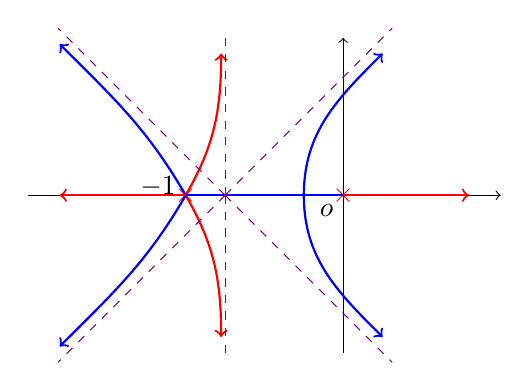
\begin{tikzpicture}[scale=2]
\coordinate (o) at (0,0);
\coordinate (ox) at (1,0);
\draw[->] (-2,0) -- (ox);
\draw[->] (0,-1) -- (0,1);
\draw (o) node[below left] {$o$};
\draw[thick,red] (-1,0) node {$\times$};
\draw[thick,red] (0,0) node {$\times$};
%\draw [red,thick,smooth] plot coordinates {(-1.8,0.96)(-1.75,0.9)(-1.2,0.3) (-1,0) (-0.9,-0.16) (-3.2/4,-0.6) (-3.1/4,-0.9) };
%\draw [red,thick,smooth] plot coordinates {(-1.8,-0.96)(-1.75,-0.9)(-1.2,-0.3) (-1,0) (-0.9,0.16) (-3.2/4,0.6) (-3.1/4,0.9) };
%\draw [red,thick,smooth] plot coordinates {(-1/4,0) (-0.9/4,0.1) (0,0.6) (1/4,0.9) };
%\draw [red,thick,smooth] plot coordinates {(-1/4,0) (-0.9/4,-0.1)(0,-0.6) (1/4,-0.9)};

\draw [->,blue,thick] (-1,0) to [out=120,in=-45] (-1.8,0.96);
\draw [->,red,thick](-1,0) to [out=-60,in=90] (-3.1/4,-0.9);
\draw [->,blue,thick] (-1,0) to [out=-120,in=45](-1.8,-0.96);
\draw [->,red,thick](-1,0) to [out=60,in=-90] (-3.1/4,0.9);
\draw [blue,thick] (-1,0)--(0,0);
\draw [->,red,thick] (0,0)--(0.8,0);
\draw [->,red,thick] (-1,0)--(-1.8,0);

\draw [->,blue,thick](-1/4,0) to [out=90,in=-135](1/4,0.9);
\draw [->,blue,thick](-1/4,0) to [out=-90,in=135](1/4,-0.9);

\draw [violet,dashed] (-3/4,0)--+(45:1.5);
\draw [violet,dashed] (-3/4,0)--+(-45:1.5);
\draw [violet,dashed] (-3/4,0)--+(135:1.5);
\draw [violet,dashed] (-3/4,0)--+(-135:1.5);

\draw [violet,dashed] (-3/4,0)--+(90:1);
\draw [violet,dashed] (-3/4,0)--+(-90:1);

%\draw (-1,0) node[below=1em] {$-1$};
\draw (-1,0) node[xshift=-1em ,yshift=0.3em] {$-1$};
\end{tikzpicture}

由根轨迹可知,$k\in(0,\frac{8}{9})$ 时,系统稳定.
}

\question(20分)单位负反馈系统开环传递函数:
$$G(s)=\frac{k}{s+1}\cdot e^{\frac{-3\pi}{4} s}$$
当 $k=1$ 时系统的稳定性如何?相角裕度是多少?若要使系统稳定,实数$k$的范围是什么?
\onlyanswer
{
答:

$|G(j\omega)|$是$\omega$的单调减函数,当$k=1,\omega=0$时,$|G(j\omega)|=1$,Nyquist曲线不包围(-1+0j),闭环系统稳定。此时$\angle G(j\omega)=0$,因此相角裕度$\gamma=180^\circ$。


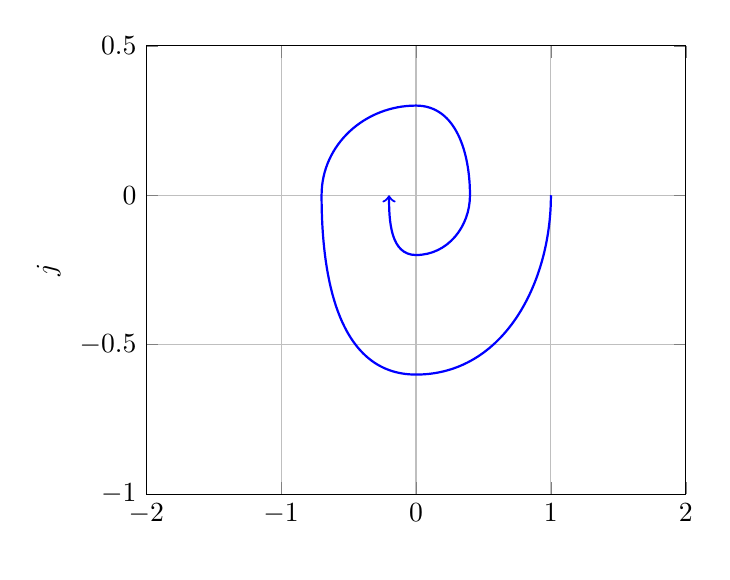
\begin{tikzpicture}[scale=1]
	\begin{axis}[
	grid=both,
	%axis x line=middle,axis y line= middle, 
	ylabel=$j$ ,xlabel=$  $ ,
	ymin=-1,ymax=0.5,xmin=-2,xmax=2,every axis plot post/.append style={mark=none}]
	%\axispath
	\draw[blue,->,thick] (axis cs:1,0)
	 to [out=-90,in=0](axis cs:0,-0.6)
	 to [out=180,in=-90](axis cs:-0.7,0)
	 to [out=90,in=180](axis cs:0,0.3)
	 to [out=0,in=90](axis cs:0.4,0)
 	 to [out=-90,in=0](axis cs:0,-0.2)
  	 to [out=180,in=-90](axis cs:-0.2,0);
	\end{axis}
\end{tikzpicture}

当$k>0,\omega=1$时, $\angle G(j\omega)=-\pi$,$|G(s)|=\frac{k}{\sqrt{2}}$,因此,当$0<k<\sqrt{2}$时,系统稳定。

当$-1<k<0$时,Nyquist曲线不包围(-1+0j),系统稳定。
当$k<-1$时,Nyquist曲线包围(-1+0j),系统不稳定。
因此,当$-1<k<\sqrt{2}$时,闭环系统稳定。


}
